\documentclass[tikz,border=5]{standalone}
\usepackage[utf8]{inputenc}

\usepackage{tikz}
\usetikzlibrary{positioning}
\usetikzlibrary{decorations.text}

\begin{document}


%------------------------------------------------------------------------------
%Introductory example
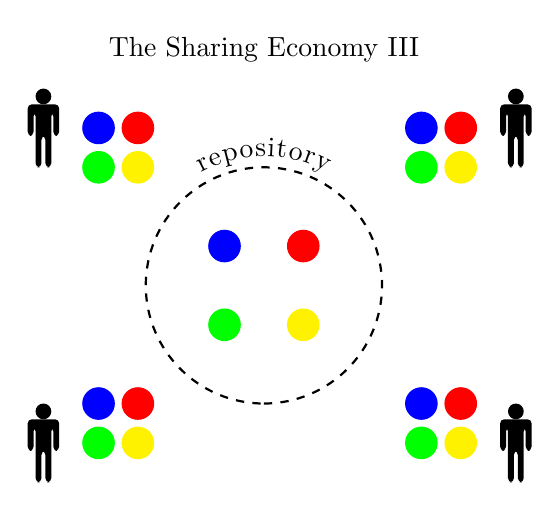
\begin{tikzpicture} 
\def\man#1;{%
    \begin{scope}[shift={#1}]
        \fill [rounded corners=1.5] (0,0.4) -- (0,0.8) -- (0.4,0.8) -- (0.4,0.4) --
            (0.325,0.4) -- (0.325,0.7) -- (0.3,0.7) -- (0.3,0) -- (0.225,0) --
            (0.225,0.4) -- (0.175,0.4) -- (0.175,0) -- (0.1,0) -- (0.1,0.7) --
            (0.075,0.7) -- (0.075,0.4) -- cycle;
        \fill (0.2,0.9) circle (0.1);
    \end{scope}}
\man(3,2);
\man(-3,-2);
\man(-3,2);
\man(3,-2);
   
\filldraw[red] (2.5,2.5) circle (0.2cm);
\filldraw[blue] (2.0,2.5) circle (0.2cm);
\filldraw[green] (2.0,2.0) circle (0.2cm);
\filldraw[yellow] (2.5,2.0) circle (0.2cm);

\filldraw[blue] (-2.1,2.5) circle (0.2cm);
\filldraw[red] (-1.6,2.5) circle (0.2cm);
\filldraw[green] (-2.1,2.0) circle (0.2cm);
\filldraw[yellow] (-1.6,2.0) circle (0.2cm);

\filldraw[green] (-2.1,-1.5) circle (0.2cm);
\filldraw[red] (-1.6,-1.0) circle (0.2cm);
\filldraw[blue] (-2.1,-1.0) circle (0.2cm);
\filldraw[yellow] (-1.6,-1.5) circle (0.2cm);

\filldraw[yellow] (2.5,-1.5) circle (0.2cm);
\filldraw[red] (2.5,-1.0) circle (0.2cm);
\filldraw[blue] (2.0,-1.0) circle (0.2cm);
\filldraw[green] (2.0,-1.5) circle (0.2cm);

\draw (0,0) node [text width=2.5cm,align=center,color=white] {Black Hole of Mediocrity}; 
\draw[thick,dashed,-latex,black,rotate=-90,postaction={decorate},decoration={text along path,
text={repository},text align=center,reverse path,raise=4pt}]
(-0.5,0) circle (1.5cm);

\node at (0,3.5) [black,fill=white]  {The Sharing Economy III} ;

\filldraw[red] (0.5,1) circle (0.2cm);
\filldraw[blue] (-0.5,1) circle (0.2cm);
\filldraw[green] (-0.5,0) circle (0.2cm);
\filldraw[yellow] (0.5,0) circle (0.2cm);


\end{tikzpicture}
%-----------------------------


\end{document}